\documentclass{article}
\usepackage[T2A]{fontenc}
\usepackage[utf8]{inputenc}
\usepackage{graphicx}
\usepackage[export]{adjustbox}
\usepackage{geometry}
\usepackage{float}
\usepackage{indentfirst}
% Preamble

% Packages
\usepackage{amsmath}

% Document
\begin{document}
    \begin{center}
    \hfill \break
    \large{МИНОБРНАУКИ РОССИИ}\\
    \footnotesize{ФЕДЕРАЛЬНОЕ ГОСУДАРСТВЕННОЕ БЮДЖЕТНОЕ ОБРАЗОВАТЕЛЬНОЕ УЧРЕЖДЕНИЕ}\\
    \footnotesize{ВЫСШЕГО ПРОФЕССИОНАЛЬНОГО ОБРАЗОВАНИЯ}\\
    \small{\textbf{«ВОРОНЕЖСКИЙ ГОСУДАРСТВЕННЫЙ УНИВЕРСИТЕТ»}}\\
    \hfill \break
    \normalsize{Факультет компьютерных наук}\\
    \hfill \break
    \normalsize{Кафедра программирования и информационных технологий}\\
    \hfill\break
    \hfill \break
    \hfill \break
    \hfill \break
    \large{Отчет по предмету Архитектура информационных систем
    \\3 лабораторная работа
    \\Приложение для автоматизированного проведения тестирования}\\
    \end{center}

    \hfill \break
    \hfill \break
    \hfill \break
    \hfill \break
    \hfill \break

    \begin{flushright} Вычиков Д.Д \end{flushright}
    \vspace*{\fill}
    \begin{center} Воронеж 2019 \end{center}
    \thispagestyle{empty}
    \newpage

    \tableofcontents

    \section{Диаграммы IDEF0}
    \subsection{Контекстная диаграмма верхнего уровня}
    \begin{figure}[H]
        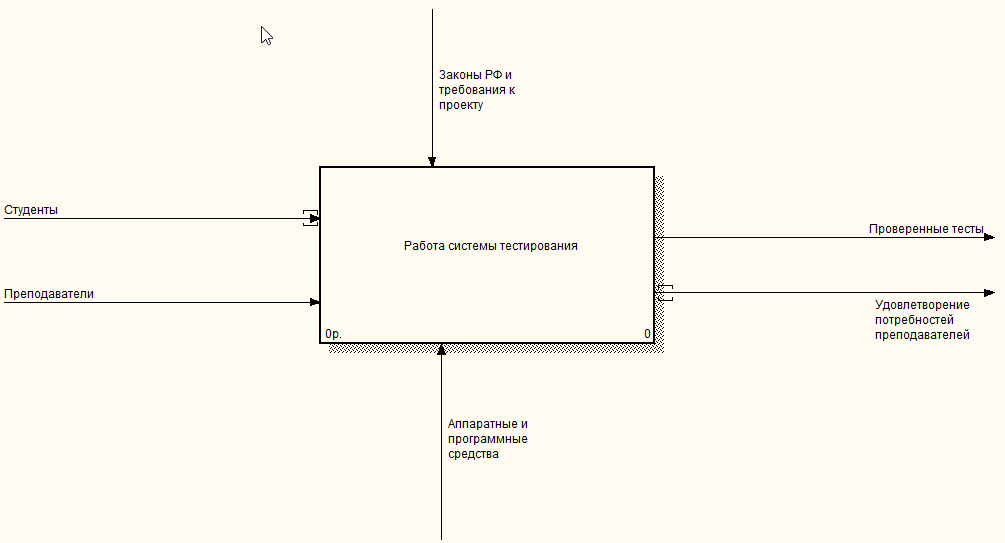
\includegraphics[width=\textwidth, center]{../img/idef0/idef0_context.png}
        \caption{Контекстная диаграмма верхнего уровня}
    \end{figure}

    Данная диаграмма является общим представлением работы автоматизированной
    системы для тестирования.

    На вход системы поступают преподаватели (администрароторы) и студенты
    (пользователи).

    Выходными блоками являются проверенные тестовые задания и удовлетворенные
    потребности преподавателей.

    Управление для данной системы осуществляют законы Российской Федерации,
    устанавливающие порядок обработки персональных данных, а также ряд других
    ограничений, и требования, предъявляемые к функциональности системы.

    Механизмами, выполняющими преобразования входных данных в выходные являются
    аппаратные и программные средства: компьютеры, операционная система,
    языки программирования, различные библиотеки и виртуальные среды для
    выполнения кода программы.

    \subsection{Работа системы тестирования}
    \begin{figure}[H]
        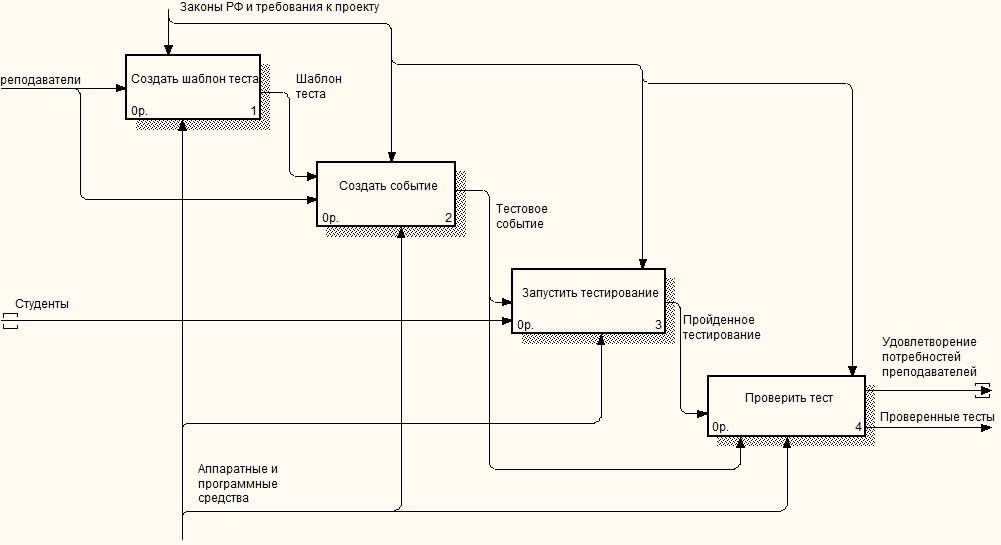
\includegraphics[width=\textwidth, center]{../img/idef0/context_decompose.png}
        \caption{Работа системы тестирования}
    \end{figure}

    Данная диаграмма раскрывает функциональный блок контекстной
    диаграммы верхнего уровня "Работа системы тестирования".

    На диаграмме представлены следующие функциональные блоки:
    \begin{enumerate}
        \item Создать шаблон теста - на вход получает преподавателей, а на выходе имеет 
        шаблон тестовый шаблон
        \item Создать событие - принимает на вход преподавателей и созданный тестовый
        шаблон и возвращает тестовое событие
        \item Запустить тестирование - получает тестовое событие и студентов, а
        выдает пройденное тестирование
        \item Проверить тест - Преобразует пройденное тестирование в проверенное
        тестирование и удовлетворение потребностей преподавателей.
    \end{enumerate}

    Далее будут более подробно рассмотрены представленные функциональные блоки.

    \subsection{Создать шаблон теста}
    \begin{figure}[H]
        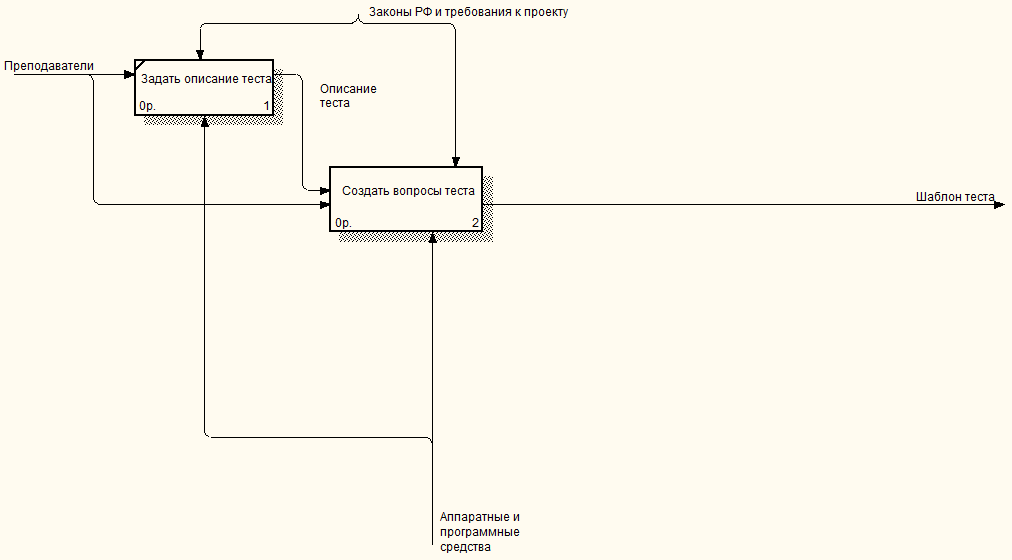
\includegraphics[width=\textwidth, center]{../img/idef0/CreateTestTemplate.png}
        \caption{Создать шаблон теста}
    \end{figure}

    На диаграмме представлены следующие функциональные блоки:
    \begin{enumerate}
        \item Задать описание теста - на вход принимает преподавателей, а на выходе
        имеет описание теста
        \item Создать вопросы теста - на вход принимает преподавателей и описание теста,
        а на выходе имеет шаблон теста
    \end{enumerate}


    \subsection{Создать вопросы теста}
    \begin{figure}[H]
        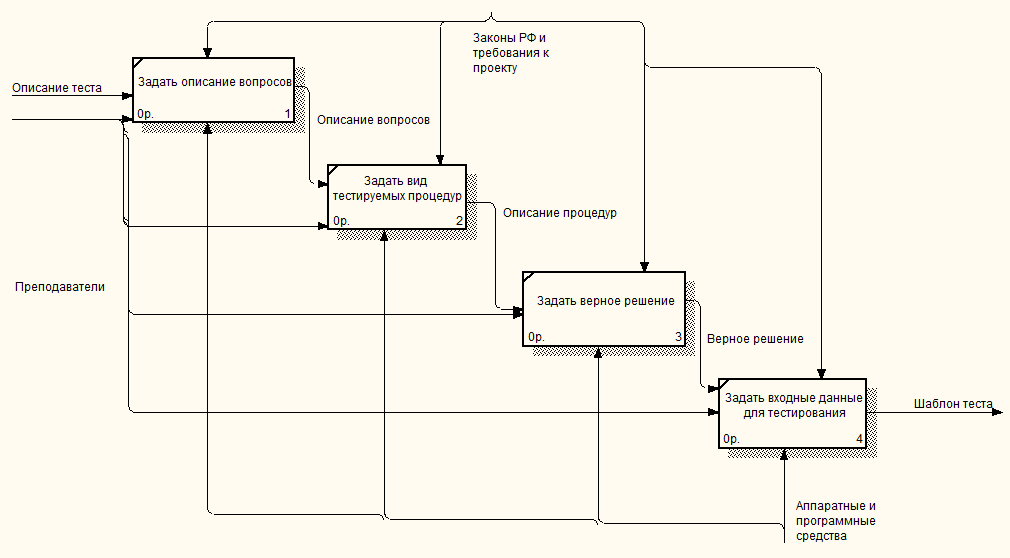
\includegraphics[width=\textwidth, center]{../img/idef0/CreateTemplateQuestions.png}
        \caption{Создать шаблон теста}
    \end{figure}
    \begin{enumerate}
        \item Задать описание вопросов - на вход принимает описание тестов и преподавателей,
        а на выходе имеет описание вопросов
        \item Задать вид тестируемых процедур - на вход принимает преподавателей и
        описание вопросов, а на выходе имеет описание процедур
        \item Задать верное решение - на вход принимает преподавателей и описание процедур,
        а на выходе имеет верное решение
        \item Задать входные данные для тестирование - на вход принимает верное решение
        и преподавателей, а на выходе имеет шаблон теста
    \end{enumerate}

    \subsection{Создать событие}
    \begin{figure}[H]
        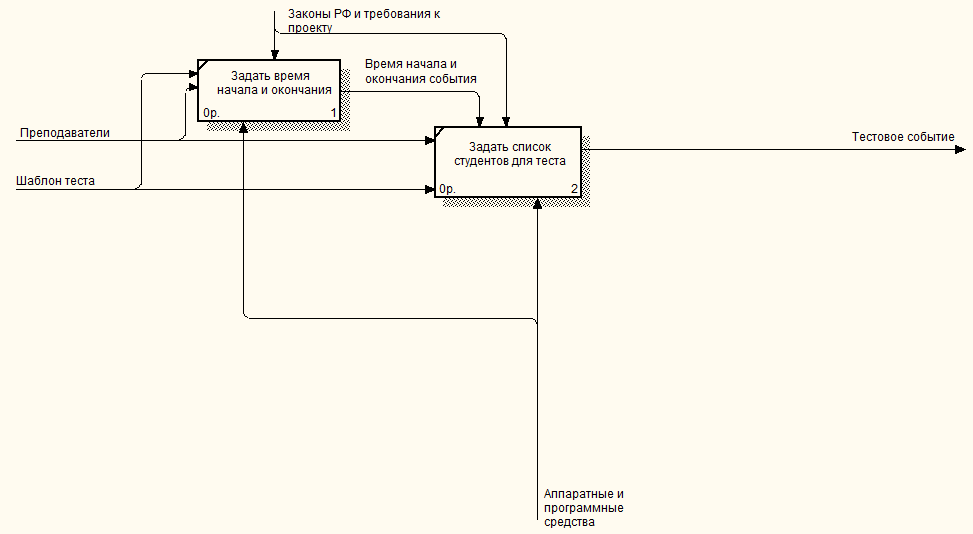
\includegraphics[width=\textwidth, center]{../img/idef0/CreateInstance.png}
        \caption{Создать событие}
    \end{figure}
    
    \begin{enumerate}
        \item Задать время начала и окончания - на вход принимает преподавателей и
        шаблон теста, а на выходе имеет время начала и окончания события
        \item Задать список студентов и для теста - на вход принимает преподавателей
        и шаблон теста, а на выходе имеет тестовое событие
    \end{enumerate}

    \subsection{Запустить тестирование}
    \begin{figure}[H]
        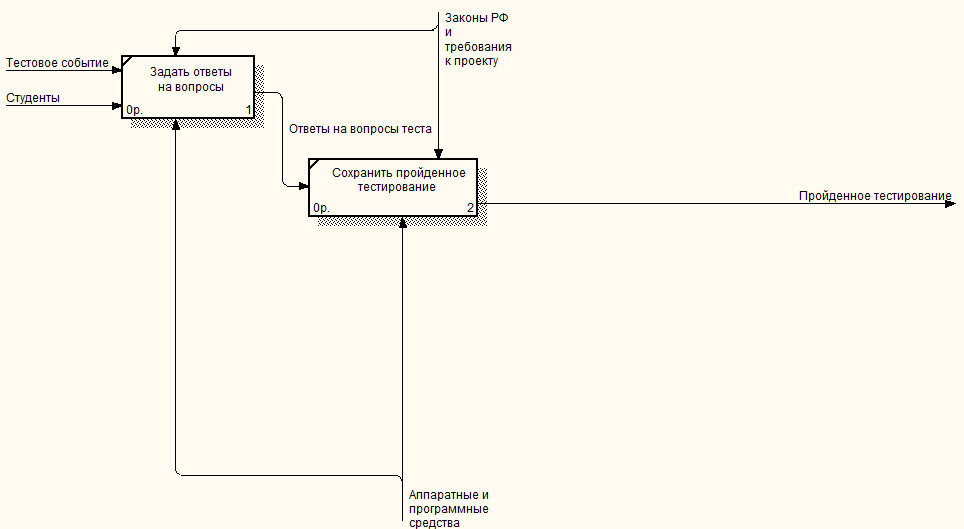
\includegraphics[width=\textwidth, center]{../img/idef0/RunTestDecompose.png}
        \caption{Запустить тестирование}
    \end{figure}

    \begin{enumerate}
        \item Задать ответы на вопросы - на вход принимает тестовое событие и
        студентов, а на выходе имеет ответы на вопросы теста
        \item Сохранить пройденное тестирование  - на вход принимает ответы
        на вопросы теста, а на выходе имеет пройденное тестирование
    \end{enumerate}

    \subsection{Проверить тест}
    \begin{figure}[H]
        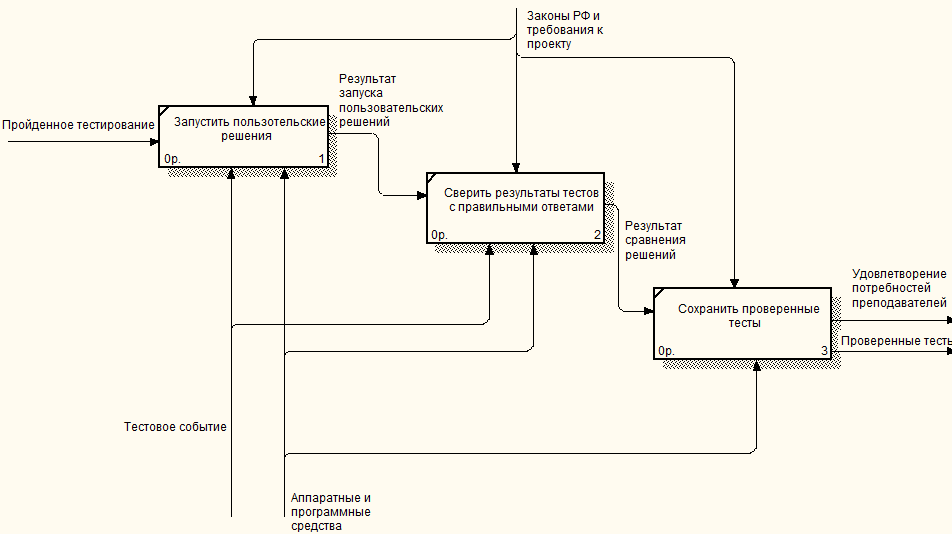
\includegraphics[width=\textwidth, center]{../img/idef0/ValidateTestDecompose.png}
        \caption{Проверить тест}
    \end{figure}

    \begin{enumerate}
        \item Запустить пользовательские решения - на вход принимает пройденное тестирование,
        а на выходе имеет результат запуска пользовательских решений
        \item Сверить результаты тестов с правильными ответами - на вход принимает 
        результат запуска пользовательских решений, а на выходе имеет результат сравнения 
        решений
        \item Сохранить проверенные тесты - на вход принимает результат сравнения
        решений, а на выходе имеет проверенные тесты и удовлетворение потребностей
        преподавателей
    \end{enumerate}
    \section{Диаграммы IDEF3}
\subsection{PFDD диаграммы}

\subsubsection{Контекстная диаграмма верхнего уровня}

Студенты и преподаватели взаимодействуют с системой,в результате чего на выходе
образуются проверенные тесты и удовлетворение потребностей преподавателей.

\begin{figure}[H]
    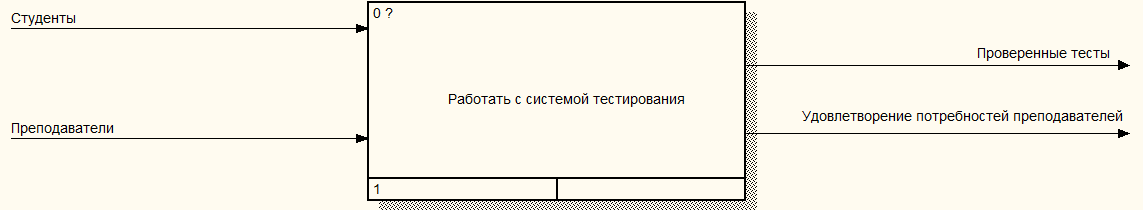
\includegraphics[width=\textwidth, center]{../img/idef3/Context.png}
    \caption{Контекстная диаграмма верхнего уровня}
\end{figure}

Данная диаграмма отображает наиболее общий вид модели системы тестирования.

\subsubsection{Работать с системой тестирования}
\begin{figure}[H]
    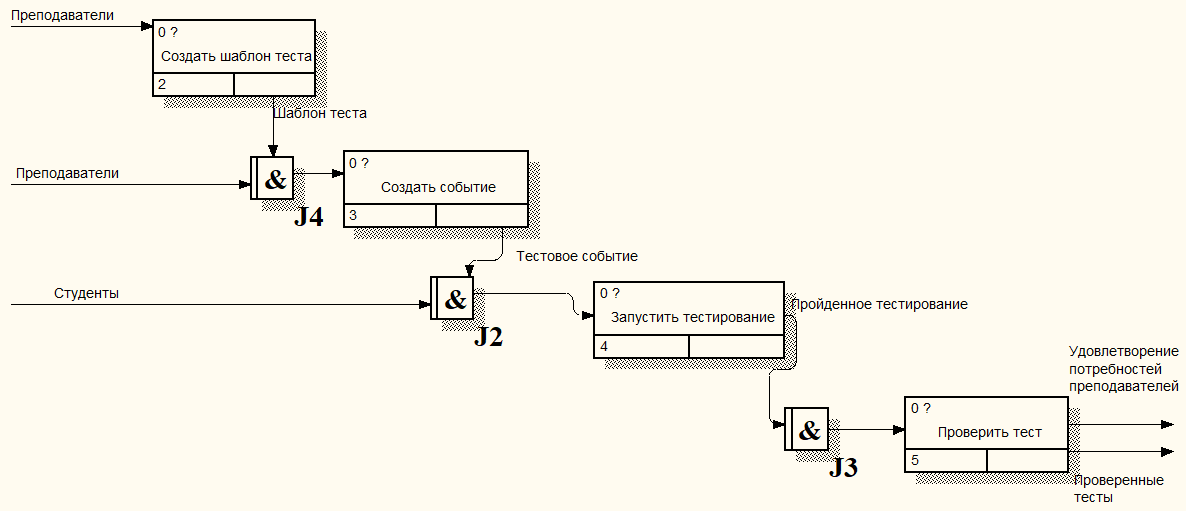
\includegraphics[width=\textwidth, center]{../img/idef3/ContextDecompose.png}
    \caption{Работать с системой тестирования}
\end{figure}

Преподаватели сначала создают шаблон теста, потом создают на основе этого шаблона
тестовое событие, которое запускают и проходят студенты, после чего пройденное 
тестирование проверяется системой на корректность, и результат проверки становится
доступен для студента, прошедшего тестирование и преподавателей.

\subsubsection{Создать шаблон теста}
\begin{figure}[H]
    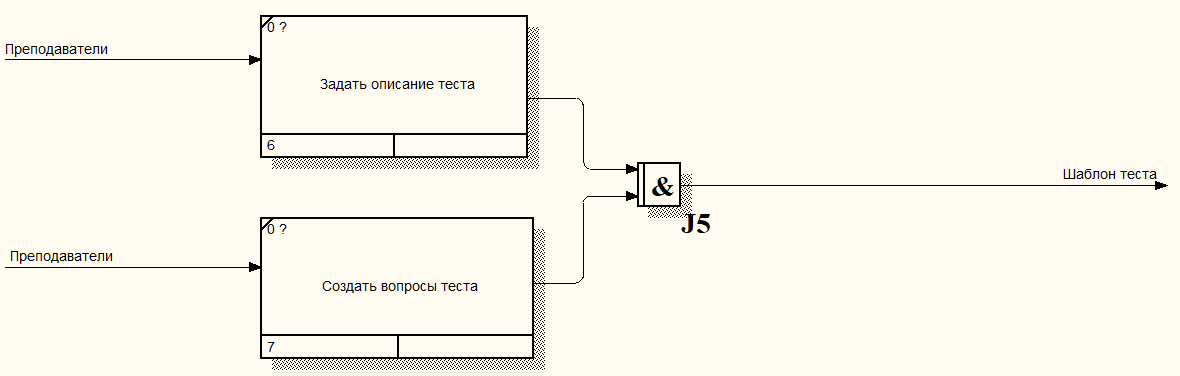
\includegraphics[width=\textwidth, center]{../img/idef3/CreateTestTemplate.png}
    \caption{Создать шаблон теста}
\end{figure}

Преподаватели задают описание теста и формируют вопросы теста, в результате чего
получает шаблон теста.

\subsubsection{Создать событие}
\begin{figure}[H]
    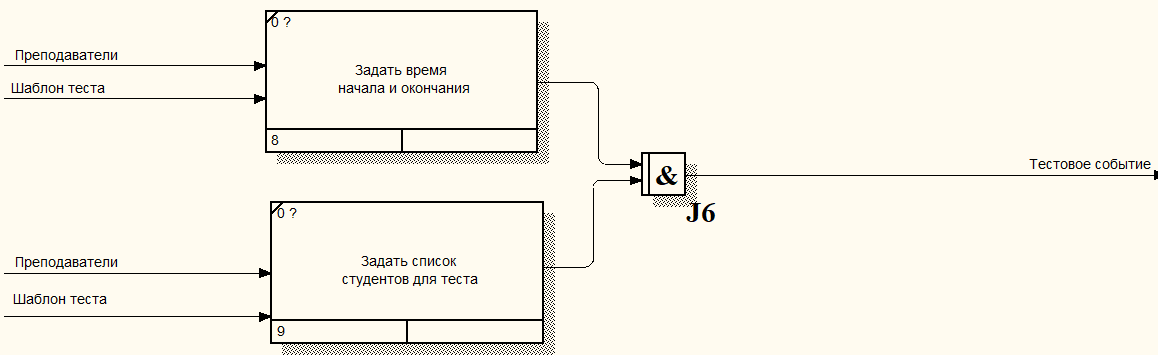
\includegraphics[width=\textwidth, center]{../img/idef3/CreateTestInstance.png}
    \caption{Создать событие}
\end{figure}

На основе шаблона теста преподаватель создает тестовое событие, для которого указывает
время начала и окончания и список студентов, которым необходимо принять участие
в этом событии.

\subsubsection{Запустить тестирование}
\begin{figure}[H]
    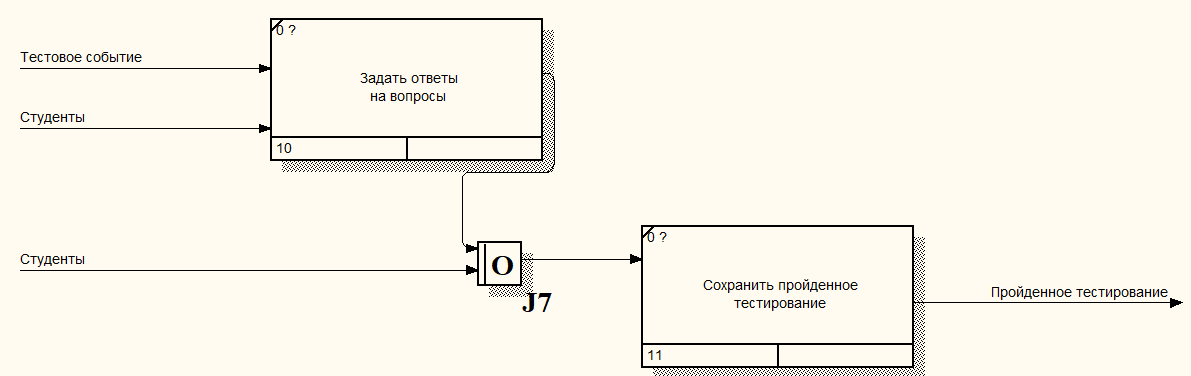
\includegraphics[width=\textwidth, center]{../img/idef3/RunTest.png}
    \caption{Запустить тестирование}
\end{figure}

Студент запускает выбранное тестовое событие и отвечает на вопросы теста,
если знает на них ответы. По завершении тестирования все ответы студента сохраняются.

\subsubsection{Проверить тестирование}
\begin{figure}[H]
    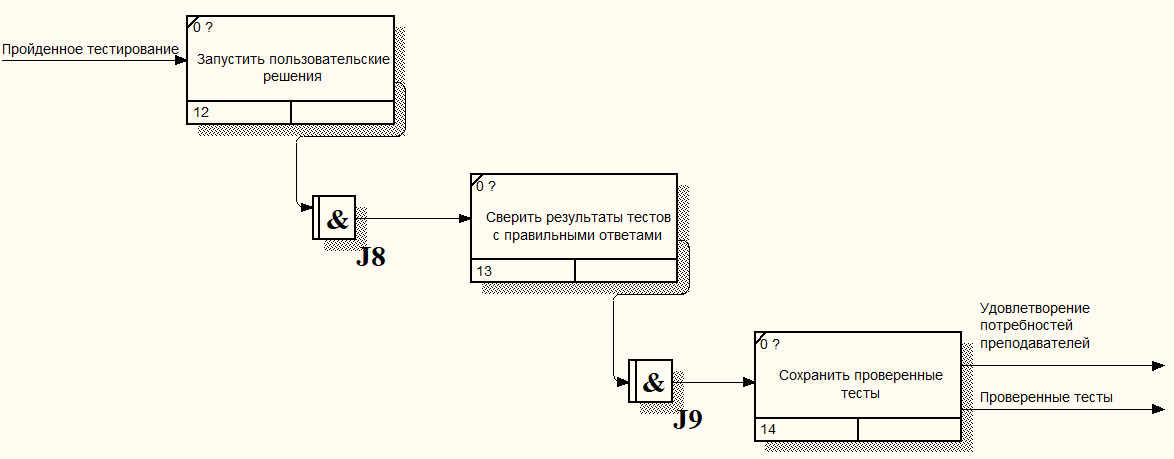
\includegraphics[width=\textwidth, center]{../img/idef3/ValidateTest.png}
    \caption{Проверить тестирование}
\end{figure}

После завершения тестирования система запускает код решений студента, получает
результаты работы алгоритмов и сравнивает их с правильными ответами на соответствующие вопросы.
После проверки результаты сохраняются и становятся доступны преподавателям и студенту,
проходившему тестирование.

\subsection{OSTN диаграмма}
\begin{figure}[H]
    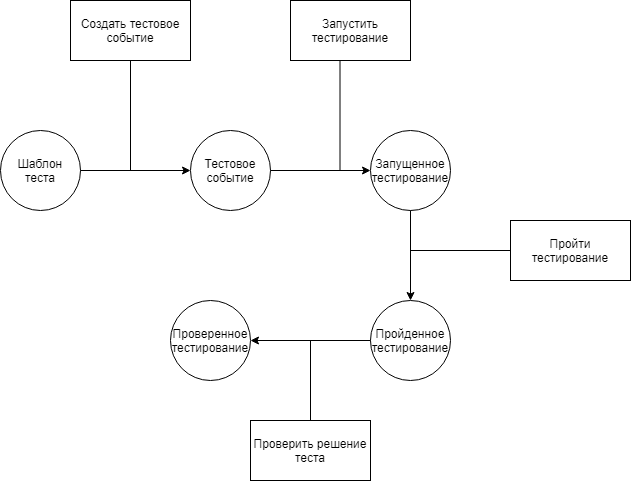
\includegraphics[width=\textwidth, center]{../img/OSTN.png}
    \caption{OSTN диаграмма}
\end{figure}

В системе не существует какого-то одного объекта, который подвергается изменениям.
Поэтому на данной диаграмме отображены основные объекты, которые присутствуют в
системе и образуются на различных этапах взаимодействия с ней.

Существуют следующие объекты:
\begin{enumerate}
    \item Шаблон теста
    \item Тестовое событие
    \item Запущенное тестирование
    \item Пройденное тестирование
    \item Проверенное тестирование
\end{enumerate}

Переходы:
\begin{enumerate}
    \item Шаблон теста -> Тестовое событие (событие создается на основе шаблона
    и имеет список назначенных на него студентов)
    \item Тестовое событие -> Запущенное тестирование (назначенный на событие студент
    может запустить его и начать проходить тестирование)
    \item Запущенное тестирование -> Пройденное тестирование (когда студент заканчивает
    прохождение тестирования, то оно становится пройденным, и его результаты сохраняются)
    \item Пройденное тестирование -> Проверенное тестирование (После прохождение тестирования
    система проверяет его и сохраняет результаты проверки)
\end{enumerate}


\subsection{DFD диаграммы}

\end{document}